\begin{figure}[htbp]
\centering
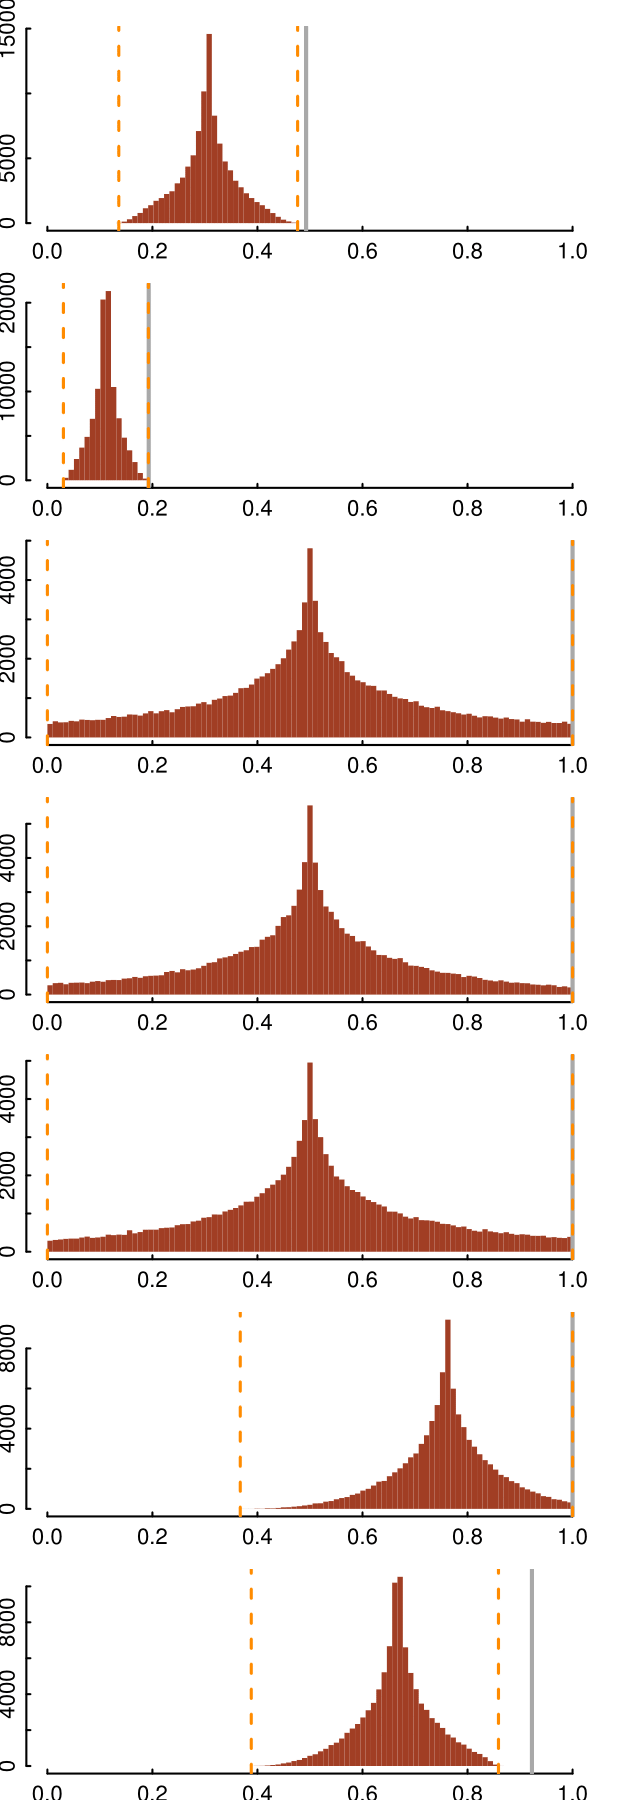
\includegraphics{sections/figs/raw_histograms.png}
\caption{Distribution of feasible activations for 50\% maximal force output in the palmar direction.}
\label{fig:raw_histograms}
\end{figure}


briantodo: add the following figures:
\begin{itemize}
\item{parcoord Full}
\item{parcoord muscle limited to 75\percent, then 50\percent, then 25\percent}
\item{}


\section{RESULTS}

Using Hit-and-Run to sample feasible activation sets, Figure \ref{fig:raw_histograms} shows the distributions of activation solutions for a palmar submaximal force.resulting from $1,000,000$ solutions computed with Hit-and-Run sampling. This is the first time (to our knowledge) that the internal structure of the feasible activation set has been visualized for a sub-maximal force.

Notice also that the lower and upper bounds of the activations (i.e., the dashed lines that indicate their bounding box), are uniquely uninformative of the actual density of distribution of feasible activations. Note also that the activation needed for the maximal force output (thick gray line) is very often not the mode of the activations at 50\% of output.


Results:
Projection onto a given muscle dimension
Simple histograms at 80% activation for one direction
Activation progression-march (3) x y z
Parallel coordinates with cost
	Full
Parallel Coordinates with cost
	Lower
	Middle
	Upper
	constraint by cost
		Yes you could put activation constraints directly in the A matrix, instead of bounds between 0 and 1. There is no advantage to adding activation constraints beforehand in the A matrix, as sampling is uniform- as long as the resulting dataset is large enough for your purpose.
		You could also put l1 and weighted l1 cost bounds as constraints in the A matrix. Cannot put higher order cost functions such as l2,l3 or weighted l2,l3.

		Talk about slopes in Parallel
		if they 

